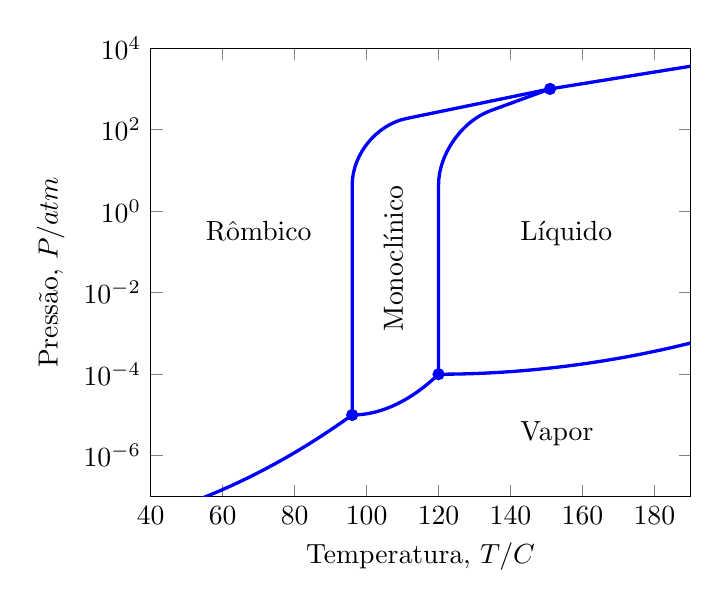
\begin{tikzpicture}
    \begin{semilogyaxis}
           [
               grid = minor,
               ylabel = {Pressão, $P/\unit{atm}$},
               xlabel = {Temperatura, $T/\unit{\degree C}$},
               ymin=0.0000001, ymax=10000,
               xmin=40, xmax=190,
           ]       
            \draw [draw=blue, very thick, rounded corners=2em]
                (axis cs: 00, 0.00000001) parabola 
                (axis cs: 96, 0.00001);
            \draw [draw=blue, very thick, rounded corners=2em]
                (axis cs: 96, 0.00001) -- 
                (axis cs: 96, 100) -- 
                (axis cs: 151, 1000);
            \draw [draw=blue, very thick]
                (axis cs: 96, 0.00001) parabola 
                (axis cs: 120, 0.0001);
            \draw [draw=blue, very thick]
                (axis cs: 120, 0.0001) parabola 
                (axis cs: 200, 0.001);
            \draw [draw=blue, very thick, rounded corners=2em]
                (axis cs: 120, 0.0001) --
                (axis cs: 120, 100) --
                (axis cs: 151, 1000);
            \draw [draw=blue, very thick, rounded corners=2em]
                (axis cs: 151, 1000) --
                (axis cs: 200, 5000);
    
            \addplot [ mark=*, color=blue, only marks ] coordinates
                { 
                    (96, 0.00001) 
                    (120, 0.0001)
                    (151, 1000)
                };
    
            \node [anchor = south west] at (axis cs: 140, 0.000001) 
                { Vapor };
            \node [anchor = north west] at (axis cs: 140, 1) 
                { Líquido };
            \node [anchor = north] at (axis cs: 70, 1) 
                { Rômbico };
            \node [rotate=90, anchor=north] at (axis cs: 102, 0.07) 
                { Monoclínico };
    \end{semilogyaxis}
    \end{tikzpicture}
    